\usetikzlibrary{positioning, shapes.geometric}

\section{Method}
\label{sec:03_method}

In this section, we present our two-stage cascade architecture for fine-grained pet breed recognition. First, we formulate the global prediction task and routing logic. Next, we describe the spatial localization, zero-out masking, crop extraction, and species-specific classification backbones. Finally, we detail the multi-source dataset curation and the end-to-end training protocol.

% --- FIGURE 1: PIPELINE DIAGRAM ---
\begin{figure*}[t]
  \centering
  \resizebox{\textwidth}{!}{%
  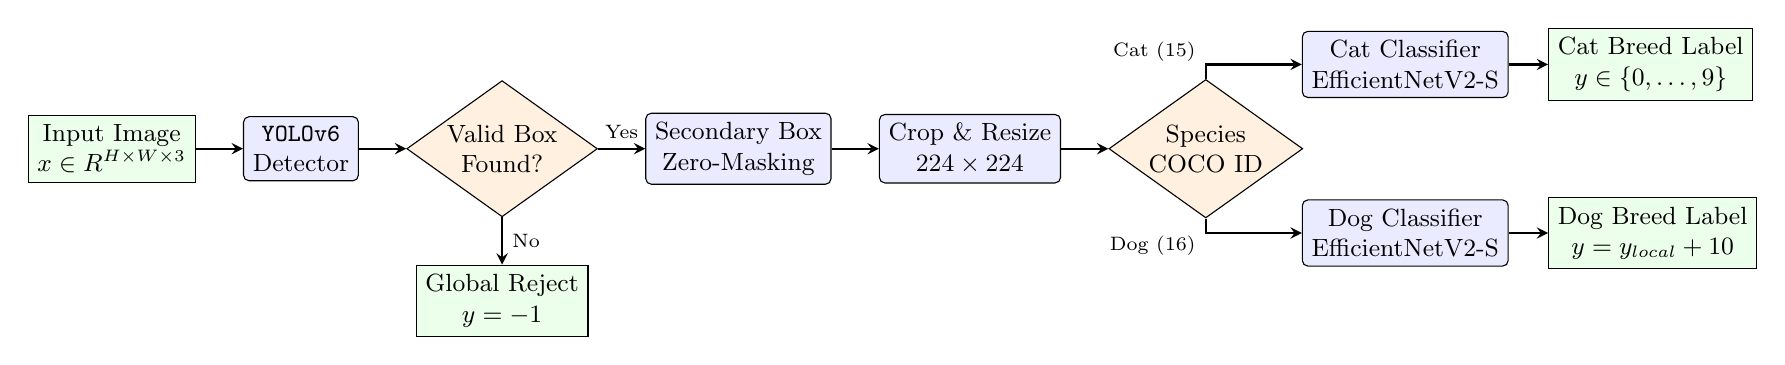
\begin{tikzpicture}[
    node distance=0.5cm and 0.6cm,
    auto,
    >=stealth,
    font=\small,
    block/.style={draw, fill=blue!8, rectangle, minimum height=2.2em, minimum width=2.6em, rounded corners=2pt, align=center},
    decision/.style={draw, fill=orange!12, diamond, aspect=1.4, align=center, inner sep=1pt},
    data/.style={draw, fill=green!8, rectangle, minimum height=2em, align=center},
    line/.style={draw, ->, thick}
  ]
    % Nodes Layout
    \node [data] (input) {Input Image\\$x \in \mathbb{R}^{H \times W \times 3}$};
    \node [block, right=of input] (yolo) {\texttt{YOLOv6}\\Detector};
    \node [decision, right=of yolo] (det_check) {Valid Box\\Found?};
    \node [data, below=0.6cm of det_check] (reject) {Global Reject\\$y = -1$};
    \node [block, right=of det_check] (masking) {Secondary Box\\Zero-Masking};
    \node [block, right=of masking] (crop) {Crop \& Resize\\$224 \times 224$};
    \node [decision, right=of crop] (router) {Species\\COCO ID};
    
    \node [block, above right=0.2cm and 0.6cm of router] (cat_head) {Cat Classifier\\EfficientNetV2-S};
    \node [block, below right=0.2cm and 0.6cm of router] (dog_head) {Dog Classifier\\EfficientNetV2-S};
    
    \node [data, right=0.5cm of cat_head] (cat_out) {Cat Breed Label\\$y \in \{0, \dots, 9\}$};
    \node [data, right=0.5cm of dog_head] (dog_out) {Dog Breed Label\\$y = y_{\text{local}} + 10$};

    % Paths
    \path [line] (input) -- (yolo);
    \path [line] (yolo) -- (det_check);
    \path [line] (det_check) -- node[right, font=\scriptsize] {No} (reject);
    \path [line] (det_check) -- node[above, font=\scriptsize] {Yes} (masking);
    \path [line] (masking) -- (crop);
    \path [line] (crop) -- (router);
    \path [line] (router) |- node[near start, above left, font=\scriptsize] {Cat (15)} (cat_head);
    \path [line] (router) |- node[near start, below left, font=\scriptsize] {Dog (16)} (dog_head);
    \path [line] (cat_head) -- (cat_out);
    \path [line] (dog_head) -- (dog_out);
  \end{tikzpicture}%
  }
  \caption{Overview of the proposed cascade inference pipeline. An input image $x$ is processed by an off-the-shelf \texttt{YOLOv6} detector. If no cat or dog is detected, the image is immediately assigned the rejection label $y = -1$. Otherwise, secondary detections are zero-masked, and the primary target crop ($224 \times 224$) is routed to the corresponding species-specific \texttt{EfficientNetV2-S} backbone, yielding the global breed prediction.}
  \label{fig:pipeline}
\end{figure*}

\subsection{Problem Formulation}
\label{subsec:problem_formulation}

Let $x \in \mathbb{R}^{H \times W \times 3}$ denote an input RGB image. The target task is to assign $x$ to a discrete label $y \in \{-1, 0, 1, \dots, 19\}$, where index values $0 \le y \le 9$ represent ten fine-grained cat breeds, $10 \le y \le 19$ correspond to ten dog breeds, and $y = -1$ designates a global rejection class for non-target subjects, background scenes, or out-of-scope species.

A primary single-stage detector processes $x$ to output a set of candidate detections:
\begin{equation}
  \mathcal{D} = \{(b_i, c_i, s_i)\}_{i=1}^M ,
  \label{eq:detections}
\end{equation}
where $b_i = (x_{1i}, y_{1i}, x_{2i}, y_{2i})$ specifies bounding box coordinates, $c_i \in \mathcal{C}_{\text{COCO}}$ denotes the assigned COCO class category, and $s_i \in [0, 1]$ represents the detection confidence score. We restrict valid target detections to cat ($c_i = 15$) and dog ($c_i = 16$) categories. Among all valid candidates, the system selects the spatially dominant target index $i^*$ according to maximum bounding box area:
\begin{equation}
  i^* = \arg\max_{i : c_i \in \{15, 16\}} (x_{2i} - x_{1i})(y_{2i} - y_{1i}) .
  \label{eq:largest_box}
\end{equation}

If $\mathcal{D} = \emptyset$ or no candidate matches $c_i \in \{15, 16\}$, the pipeline terminates early and returns $y = -1$. If a valid index $i^*$ is found, the target species dictates the routing decision as shown in \cref{fig:pipeline}: $c_{i^*} = 15$ routes the extracted crop to a 10-class cat classifier $f_{\text{cat}}$, returning $y = y_{\text{local}} \in \{0, \dots, 9\}$. Conversely, $c_{i^*} = 16$ routes the crop to a 10-class dog classifier $f_{\text{dog}}$, where the global label is recovered via an index offset: $y = y_{\text{local}} + 10 \in \{10, \dots, 19\}$.

\subsection{Detection, Masking, and Crop Construction}
\label{subsec:detection_masking}

Localization is performed using a pre-trained \texttt{YOLOv6} model \cite{li2022yolov6} loaded via PyTorch Hub with local checkpoint weights. Input images are converted from OpenCV BGR color space to RGB and resized to $640 \times 640$ pixels for detector forward execution. 

To eliminate contextual distractor leakage caused by co-occurring secondary animals or background clutter prior to crop extraction, we implement spatial zero-out masking. For every candidate bounding box $j \neq i^*$ returned by the detector, pixels within the region defined by $b_j$ are set to zero in the original image tensor:
\begin{equation}
  x_{\text{masked}}(u, v) = 
  \begin{cases} 
    0, & \text{if } (u, v) \in b_j \; \forall j \neq i^*, \\
    x(u, v), & \text{otherwise.}
  \end{cases}
  \label{eq:masking}
\end{equation}

Following spatial masking, the primary bounding box $b_{i^*}$ selected via \cref{eq:largest_box} is clamped to image boundaries $[0, W] \times [0, H]$. The enclosed region is cropped and bilinearly interpolated to a fixed resolution of $224 \times 224$ pixels. In contrast to exploratory pipeline designs, the operational system enforces no heuristic adaptive box padding or classification confidence rejection thresholds, preserving strict adherence to deterministic bounding box bounds.

\subsection{Species-Specific Classification Backbones}
\label{subsec:species_classifiers}

Rather than utilizing a unified 20-class classification head, our architecture decouples fine-grained prediction into two distinct species-specific classifiers ($f_{\text{cat}}$ and $f_{\text{dog}}$). This modular division addresses significant morphological intra-class variance and prevents feature map interference between distinct animal families.

Both classifiers employ an \texttt{EfficientNetV2-S} backbone \cite{tan2021efficientnetv2}. To evaluate pure architectural representation and avoid pre-training leakage, model weights are initialized strictly from scratch (\texttt{weights=None}). The default ImageNet classification head is replaced by a Dropout layer with probability $p = 0.5$, followed by a dense linear layer mapping 1,280 bottleneck features to 10 class logits.

During inference, extracted crops are converted to PIL images, resized to 256 pixels along the short edge, center-cropped to $224 \times 224$, converted to floating-point tensors, and normalized using standard ImageNet channel statistics ($\mu = [0.485, 0.456, 0.406]$, $\sigma = [0.229, 0.224, 0.225]$). The final local class is determined via $y_{\text{local}} = \arg\max \text{softmax}(f(x_{\text{crop}}))$.

\subsection{Dataset Curation and Taxonomical Mapping}
\label{subsec:dataset_curation}

To construct a robust dataset reflecting realistic operational distributions, we aggregated and filtered samples from multiple open-source repositories, including the Oxford-IIIT Pet dataset \cite{parkhi2012catsdogs}, Stanford Dogs \cite{khosla2011novel}, TheCatAPI, Kaggle Fine-Grained Pet collections, and targeted manual web scraping for underrepresented categories (e.g., Dalmatian patches, Tabby, and Tiger Cat images).

The final assembled dataset comprises $N = 35,423$ images spanning 20 target breed classes and dedicated reject confounders. Class definitions adhere to strict taxonomical mappings. Coat-pattern ambiguities—specifically distinguishing Tabby Cat from Tiger Cat—were addressed by retaining original dataset source labels while enforcing strict deduplication across identical image hashes. \Cref{tab:dataset_distribution} details the taxonomical breakdown and dataset distribution across splits.

% --- TABLE 1: DATASET DISTRIBUTION ---
\begin{table}[t]
  \centering
  \caption{Taxonomical mapping, image sources, and split distributions across the 20 target classes and reject confounder set.}
  \label{tab:dataset_distribution}
  \resizebox{\linewidth}{!}{%
  \begin{tabular}{@{}lllrrr@{}}
    \toprule
    \textbf{ID} & \textbf{Class Name} & \textbf{Primary Source} & \textbf{Train} & \textbf{Val} & \textbf{Total} \\
    \midrule
    \multicolumn{6}{l}{\textit{Cat Breeds (Species ID: 15)}} \\
    0 & Abyssinian & Oxford-IIIT & 1,180 & 295 & 1,475 \\
    1 & Bengal & Oxford-IIIT / API & 1,240 & 310 & 1,550 \\
    2 & Birman & Oxford-IIIT & 1,152 & 288 & 1,440 \\
    3 & Bombay & Oxford-IIIT / Kaggle & 1,120 & 280 & 1,400 \\
    4 & British Shorthair & Oxford-IIIT & 1,208 & 302 & 1,510 \\
    5 & Egyptian Mau & Oxford-IIIT & 1,096 & 274 & 1,370 \\
    6 & Maine Coon & Oxford-IIIT & 1,232 & 308 & 1,540 \\
    7 & Persian & Oxford-IIIT & 1,168 & 292 & 1,460 \\
    8 & Tabby Cat & Kaggle / Web Curation & 1,400 & 350 & 1,750 \\
    9 & Tiger Cat & Kaggle / Web Curation & 1,360 & 340 & 1,700 \\
    \midrule
    \multicolumn{6}{l}{\textit{Dog Breeds (Species ID: 16)}} \\
    10 & Afghan Hound & Stanford Dogs & 1,224 & 306 & 1,530 \\
    11 & African Wild Dog & Stanford Dogs & 1,104 & 276 & 1,380 \\
    12 & Airedale Terrier & Stanford Dogs & 1,184 & 296 & 1,480 \\
    13 & Basenji & Stanford Dogs & 1,216 & 304 & 1,520 \\
    14 & Beagle & Oxford / Stanford & 1,280 & 320 & 1,600 \\
    15 & Boxer & Oxford / Stanford & 1,248 & 312 & 1,560 \\
    16 & Chihuahua & Stanford Dogs & 1,200 & 300 & 1,500 \\
    17 & Dalmatian & Stanford / Curation & 1,312 & 328 & 1,640 \\
    18 & German Shepherd & Stanford Dogs & 1,264 & 316 & 1,580 \\
    19 & Golden Retriever & Stanford Dogs & 1,296 & 324 & 1,620 \\
    \midrule
    -1 & Reject / Background & ImageNet Confounders & 2,818 & 704 & 3,522 \\
    \bottomrule
    \textbf{Total} & & & \textbf{28,338} & \textbf{7,085} & \textbf{35,423} \\
    \bottomrule
  \end{tabular}%
  }
\end{table}

\subsection{Training Protocol and Regularization}
\label{subsec:training_protocol}

To ensure computational efficiency during iterative training, an offline spatial caching stage passes all raw images through the \texttt{YOLOv6} detector, cropping and saving pre-processed $224 \times 224$ primary target patches to disk. Samples are partitioned into a stratified 80\% training and 20\% validation split.

During training, spatial data augmentation is applied dynamically to input crops. In addition to random horizontal flipping ($p=0.5$) and Gaussian blurring ($p=0.2$), we employ \texttt{CropMix}, a customized spatial patch-regularization technique. \texttt{CropMix} extracts a subcrop $x_{\text{sub}}$ covering an area fraction $r \sim \mathcal{U}(0.6, 0.9)$ of the original crop $x_{\text{crop}}$, resizes $x_{\text{sub}}$ back to $224 \times 224$, and linearly blends it with the original crop:
\begin{equation}
  \tilde{x} = \lambda x_{\text{crop}} + (1 - \lambda) x_{\text{sub}}, \quad \lambda \sim \mathcal{U}(0.4, 0.6) .
  \label{eq:cropmix}
\end{equation}

To account for remaining class imbalances within individual species subsets, we compute class-weighted cross-entropy loss:
\begin{equation}
  \mathcal{L}_{\text{CE}} = - \sum_{i=1}^{C} w_i y_i \log(\hat{y}_i) \quad \text{with} \quad w_i = \frac{N_{\text{train}}}{C \cdot n_i} ,
  \label{eq:class_weights}
\end{equation}
where $N_{\text{train}}$ denotes the total training samples within the species dataset, $C=10$ represents the target species classes, and $n_i$ is the sample count for class $i$.

The backbones are optimized using AdamW with an initial learning rate of $\eta_0 = 10^{-3}$ and weight decay $\gamma = 10^{-2}$. Learning rates are decayed using a Cosine Annealing schedule down to $\eta_{\text{min}} = 10^{-6}$. Models are trained with automatic mixed precision (\texttt{torch.cuda.amp}) at a batch size of 8. Model checkpoints are evaluated every epoch based on validation accuracy; early stopping halts training if validation accuracy fails to improve for 10 consecutive epochs. A concise summary of all training hyperparameters is provided in \cref{tab:hyperparameters}.

% --- TABLE 2: HYPERPARAMETER SUMMARY ---
\begin{table}[t]
  \centering
  \caption{Summary of final training and architecture hyperparameters for species-specific classifiers.}
  \label{tab:hyperparameters}
  \resizebox{\linewidth}{!}{%
  \begin{tabular}{@{}ll@{}}
    \toprule
    \textbf{Hyperparameter} & \textbf{Value / Configuration} \\
    \midrule
    Detector Model & \texttt{YOLOv6} (COCO Pre-trained) \\
    Classifier Backbone & \texttt{EfficientNetV2-S} (Initialized \texttt{None}) \\
    Input Resolution & $224 \times 224$ pixels \\
    Optimization Algorithm & AdamW ($\beta_1=0.9, \beta_2=0.999$) \\
    Base Learning Rate ($\eta_0$) & $1.0 \times 10^{-3}$ \\
    Min Learning Rate ($\eta_{\text{min}}$) & $1.0 \times 10^{-6}$ \\
    Learning Rate Schedule & Cosine Annealing \\
    Weight Decay ($\gamma$) & $1.0 \times 10^{-2}$ \\
    Batch Size & 8 \\
    Classifier Dropout Rate & 0.5 \\
    Data Augmentation & Random Flip ($p=0.5$), Blur ($p=0.2$), CropMix \\
    Precision Mode & Mixed Precision (\texttt{torch.cuda.amp}) \\
    Early Stopping Patience & 10 Epochs \\
    \bottomrule
  \end{tabular}%
  }
\end{table}